
%% bare_jrnl.tex
%% V1.4
%% 2012/12/27
%% by Michael Shell
%% see http://www.michaelshell.org/
%% for current contact information.
%%
%% This is a skeleton file demonstrating the use of IEEEtran.cls
%% (requires IEEEtran.cls version 1.8 or later) with an IEEE journal paper.
%%
%% Support sites:
%% http://www.michaelshell.org/tex/ieeetran/
%% http://www.ctan.org/tex-archive/macros/latex/contrib/IEEEtran/
%% and
%% http://www.ieee.org/


% *** Authors should verify (and, if needed, correct) their LaTeX system  ***
% *** with the testflow diagnostic prior to trusting their LaTeX platform ***
% *** with production work. IEEE's font choices can trigger bugs that do  ***
% *** not appear when using other class files.                            ***
% The testflow support page is at:
% http://www.michaelshell.org/tex/testflow/


%%*************************************************************************
%% Legal Notice:
%% This code is offered as-is without any warranty either expressed or
%% implied; without even the implied warranty of MERCHANTABILITY or
%% FITNESS FOR A PARTICULAR PURPOSE! 
%% User assumes all risk.
%% In no event shall IEEE or any contributor to this code be liable for
%% any damages or losses, including, but not limited to, incidental,
%% consequential, or any other damages, resulting from the use or misuse
%% of any information contained here.
%%
%% All comments are the opinions of their respective authors and are not
%% necessarily endorsed by the IEEE.
%%
%% This work is distributed under the LaTeX Project Public License (LPPL)
%% ( http://www.latex-project.org/ ) version 1.3, and may be freely used,
%% distributed and modified. A copy of the LPPL, version 1.3, is included
%% in the base LaTeX documentation of all distributions of LaTeX released
%% 2003/12/01 or later.
%% Retain all contribution notices and credits.
%% ** Modified files should be clearly indicated as such, including  **
%% ** renaming them and changing author support contact information. **
%%
%% File list of work: IEEEtran.cls, IEEEtran_HOWTO.pdf, bare_adv.tex,
%%                    bare_conf.tex, bare_jrnl.tex, bare_jrnl_compsoc.tex,
%%                    bare_jrnl_transmag.tex
%%*************************************************************************

% Note that the a4paper option is mainly intended so that authors in
% countries using A4 can easily print to A4 and see how their papers will
% look in print - the typesetting of the document will not typically be
% affected with changes in paper size (but the bottom and side margins will).
% Use the testflow package mentioned above to verify correct handling of
% both paper sizes by the user's LaTeX system.
%
% Also note that the "draftcls" or "draftclsnofoot", not "draft", option
% should be used if it is desired that the figures are to be displayed in
% draft mode.
%
\documentclass[journal]{IEEEtran}
%
% If IEEEtran.cls has not been installed into the LaTeX system files,
% manually specify the path to it like:
% \documentclass[journal]{../sty/IEEEtran}

\usepackage[justification=centering]{caption}


% Some very useful LaTeX packages include:
% (uncomment the ones you want to load)

\usepackage{xcolor}

% *** MISC UTILITY PACKAGES ***
%
%\usepackage{ifpdf}
% Heiko Oberdiek's ifpdf.sty is very useful if you need conditional
% compilation based on whether the output is pdf or dvi.
% usage:
% \ifpdf
%   % pdf code
% \else
%   % dvi code
% \fi
% The latest version of ifpdf.sty can be obtained from:
% http://www.ctan.org/tex-archive/macros/latex/contrib/oberdiek/
% Also, note that IEEEtran.cls V1.7 and later provides a builtin
% \ifCLASSINFOpdf conditional that works the same way.
% When switching from latex to pdflatex and vice-versa, the compiler may
% have to be run twice to clear warning/error messages.




% *** CITATION PACKAGES ***
%
%\usepackage{cite}
% cite.sty was written by Donald Arseneau
% V1.6 and later of IEEEtran pre-defines the format of the cite.sty package
% \cite{} output to follow that of IEEE. Loading the cite package will
% result in citation numbers being automatically sorted and properly
% "compressed/ranged". e.g., [1], [9], [2], [7], [5], [6] without using
% cite.sty will become [1], [2], [5]--[7], [9] using cite.sty. cite.sty's
% \cite will automatically add leading space, if needed. Use cite.sty's
% noadjust option (cite.sty V3.8 and later) if you want to turn this off
% such as if a citation ever needs to be enclosed in parenthesis.
% cite.sty is already installed on most LaTeX systems. Be sure and use
% version 4.0 (2003-05-27) and later if using hyperref.sty. cite.sty does
% not currently provide for hyperlinked citations.
% The latest version can be obtained at:
% http://www.ctan.org/tex-archive/macros/latex/contrib/cite/
% The documentation is contained in the cite.sty file itself.



% *** GRAPHICS RELATED PACKAGES ***
%
\ifCLASSINFOpdf
   \usepackage[pdftex]{graphicx}
  % declare the path(s) where your graphic files are
  % \graphicspath{{../pdf/}{../jpeg/}}
  % and their extensions so you won't have to specify these with
  % every instance of \includegraphics
  % \DeclareGraphicsExtensions{.pdf,.jpeg,.png}
\else
  % or other class option (dvipsone, dvipdf, if not using dvips). graphicx
  % will default to the driver specified in the system graphics.cfg if no
  % driver is specified.
   \usepackage[dvips]{graphicx}
  % declare the path(s) where your graphic files are
  % \graphicspath{{../eps/}}
  % and their extensions so you won't have to specify these with
  % every instance of \includegraphics
  % \DeclareGraphicsExtensions{.eps}
\fi
% graphicx was written by David Carlisle and Sebastian Rahtz. It is
% required if you want graphics, photos, etc. graphicx.sty is already
% installed on most LaTeX systems. The latest version and documentation
% can be obtained at: 
% http://www.ctan.org/tex-archive/macros/latex/required/graphics/
% Another good source of documentation is "Using Imported Graphics in
% LaTeX2e" by Keith Reckdahl which can be found at:
% http://www.ctan.org/tex-archive/info/epslatex/
%
% latex, and pdflatex in dvi mode, support graphics in encapsulated
% postscript (.eps) format. pdflatex in pdf mode supports graphics
% in .pdf, .jpeg, .png and .mps (metapost) formats. Users should ensure
% that all non-photo figures use a vector format (.eps, .pdf, .mps) and
% not a bitmapped formats (.jpeg, .png). IEEE frowns on bitmapped formats
% which can result in "jaggedy"/blurry rendering of lines and letters as
% well as large increases in file sizes.
%
% You can find documentation about the pdfTeX application at:
% http://www.tug.org/applications/pdftex



% *** MATH PACKAGES ***
%
\usepackage[cmex10]{amsmath}
% A popular package from the American Mathematical Society that provides
% many useful and powerful commands for dealing with mathematics. If using
% it, be sure to load this package with the cmex10 option to ensure that
% only type 1 fonts will utilized at all point sizes. Without this option,
% it is possible that some math symbols, particularly those within
% footnotes, will be rendered in bitmap form which will result in a
% document that can not be IEEE Xplore compliant!
%
% Also, note that the amsmath package sets \interdisplaylinepenalty to 10000
% thus preventing page breaks from occurring within multiline equations. Use:
%\interdisplaylinepenalty=2500
% after loading amsmath to restore such page breaks as IEEEtran.cls normally
% does. amsmath.sty is already installed on most LaTeX systems. The latest
% version and documentation can be obtained at:
% http://www.ctan.org/tex-archive/macros/latex/required/amslatex/math/




% *** SPECIALIZED LIST PACKAGES ***
%
%\usepackage{algorithmic}
% algorithmic.sty was written by Peter Williams and Rogerio Brito.
% This package provides an algorithmic environment fo describing algorithms.
% You can use the algorithmic environment in-text or within a figure
% environment to provide for a floating algorithm. Do NOT use the algorithm
% floating environment provided by algorithm.sty (by the same authors) or
% algorithm2e.sty (by Christophe Fiorio) as IEEE does not use dedicated
% algorithm float types and packages that provide these will not provide
% correct IEEE style captions. The latest version and documentation of
% algorithmic.sty can be obtained at:
% http://www.ctan.org/tex-archive/macros/latex/contrib/algorithms/
% There is also a support site at:
% http://algorithms.berlios.de/index.html
% Also of interest may be the (relatively newer and more customizable)
% algorithmicx.sty package by Szasz Janos:
% http://www.ctan.org/tex-archive/macros/latex/contrib/algorithmicx/




% *** ALIGNMENT PACKAGES ***
%
%\usepackage{array}
% Frank Mittelbach's and David Carlisle's array.sty patches and improves
% the standard LaTeX2e array and tabular environments to provide better
% appearance and additional user controls. As the default LaTeX2e table
% generation code is lacking to the point of almost being broken with
% respect to the quality of the end results, all users are strongly
% advised to use an enhanced (at the very least that provided by array.sty)
% set of table tools. array.sty is already installed on most systems. The
% latest version and documentation can be obtained at:
% http://www.ctan.org/tex-archive/macros/latex/required/tools/


% IEEEtran contains the IEEEeqnarray family of commands that can be used to
% generate multiline equations as well as matrices, tables, etc., of high
% quality.


% *** SUBFIGURE PACKAGES ***
%\ifCLASSOPTIONcompsoc
%  \usepackage[caption=false,font=normalsize,labelfont=sf,textfont=sf]{subfig}
%\else
%  \usepackage[caption=false,font=footnotesize]{subfig}
%\fi
% subfig.sty, written by Steven Douglas Cochran, is the modern replacement
% for subfigure.sty, the latter of which is no longer maintained and is
% incompatible with some LaTeX packages including fixltx2e. However,
% subfig.sty requires and automatically loads Axel Sommerfeldt's caption.sty
% which will override IEEEtran.cls' handling of captions and this will result
% in non-IEEE style figure/table captions. To prevent this problem, be sure
% and invoke subfig.sty's "caption=false" package option (available since
% subfig.sty version 1.3, 2005/06/28) as this is will preserve IEEEtran.cls
% handling of captions.
% Note that the Computer Society format requires a larger sans serif font
% than the serif footnote size font used in traditional IEEE formatting
% and thus the need to invoke different subfig.sty package options depending
% on whether compsoc mode has been enabled.
%
% The latest version and documentation of subfig.sty can be obtained at:
% http://www.ctan.org/tex-archive/macros/latex/contrib/subfig/




% *** FLOAT PACKAGES ***
%
%\usepackage{fixltx2e}
% fixltx2e, the successor to the earlier fix2col.sty, was written by
% Frank Mittelbach and David Carlisle. This package corrects a few problems
% in the LaTeX2e kernel, the most notable of which is that in current
% LaTeX2e releases, the ordering of single and double column floats is not
% guaranteed to be preserved. Thus, an unpatched LaTeX2e can allow a
% single column figure to be placed prior to an earlier double column
% figure. The latest version and documentation can be found at:
% http://www.ctan.org/tex-archive/macros/latex/base/


%\usepackage{stfloats}
% stfloats.sty was written by Sigitas Tolusis. This package gives LaTeX2e
% the ability to do double column floats at the bottom of the page as well
% as the top. (e.g., "\begin{figure*}[!b]" is not normally possible in
% LaTeX2e). It also provides a command:
%\fnbelowfloat
% to enable the placement of footnotes below bottom floats (the standard
% LaTeX2e kernel puts them above bottom floats). This is an invasive package
% which rewrites many portions of the LaTeX2e float routines. It may not work
% with other packages that modify the LaTeX2e float routines. The latest
% version and documentation can be obtained at:
% http://www.ctan.org/tex-archive/macros/latex/contrib/sttools/
% Do not use the stfloats baselinefloat ability as IEEE does not allow
% \baselineskip to stretch. Authors submitting work to the IEEE should note
% that IEEE rarely uses double column equations and that authors should try
% to avoid such use. Do not be tempted to use the cuted.sty or midfloat.sty
% packages (also by Sigitas Tolusis) as IEEE does not format its papers in
% such ways.
% Do not attempt to use stfloats with fixltx2e as they are incompatible.
% Instead, use Morten Hogholm'a dblfloatfix which combines the features
% of both fixltx2e and stfloats:
%
% \usepackage{dblfloatfix}
% The latest version can be found at:
% http://www.ctan.org/tex-archive/macros/latex/contrib/dblfloatfix/




%\ifCLASSOPTIONcaptionsoff
%  \usepackage[nomarkers]{endfloat}
% \let\MYoriglatexcaption\caption
% \renewcommand{\caption}[2][\relax]{\MYoriglatexcaption[#2]{#2}}
%\fi
% endfloat.sty was written by James Darrell McCauley, Jeff Goldberg and 
% Axel Sommerfeldt. This package may be useful when used in conjunction with 
% IEEEtran.cls'  captionsoff option. Some IEEE journals/societies require that
% submissions have lists of figures/tables at the end of the paper and that
% figures/tables without any captions are placed on a page by themselves at
% the end of the document. If needed, the draftcls IEEEtran class option or
% \CLASSINPUTbaselinestretch interface can be used to increase the line
% spacing as well. Be sure and use the nomarkers option of endfloat to
% prevent endfloat from "marking" where the figures would have been placed
% in the text. The two hack lines of code above are a slight modification of
% that suggested by in the endfloat docs (section 8.4.1) to ensure that
% the full captions always appear in the list of figures/tables - even if
% the user used the short optional argument of \caption[]{}.
% IEEE papers do not typically make use of \caption[]'s optional argument,
% so this should not be an issue. A similar trick can be used to disable
% captions of packages such as subfig.sty that lack options to turn off
% the subcaptions:
% For subfig.sty:
% \let\MYorigsubfloat\subfloat
% \renewcommand{\subfloat}[2][\relax]{\MYorigsubfloat[]{#2}}
% However, the above trick will not work if both optional arguments of
% the \subfloat command are used. Furthermore, there needs to be a
% description of each subfigure *somewhere* and endfloat does not add
% subfigure captions to its list of figures. Thus, the best approach is to
% avoid the use of subfigure captions (many IEEE journals avoid them anyway)
% and instead reference/explain all the subfigures within the main caption.
% The latest version of endfloat.sty and its documentation can obtained at:
% http://www.ctan.org/tex-archive/macros/latex/contrib/endfloat/
%
% The IEEEtran \ifCLASSOPTIONcaptionsoff conditional can also be used
% later in the document, say, to conditionally put the References on a 
% page by themselves.




% *** PDF, URL AND HYPERLINK PACKAGES ***
%
\usepackage{url}
% url.sty was written by Donald Arseneau. It provides better support for
% handling and breaking URLs. url.sty is already installed on most LaTeX
% systems. The latest version and documentation can be obtained at:
% http://www.ctan.org/tex-archive/macros/latex/contrib/url/
% Basically, \url{my_url_here}.



% *** Do not adjust lengths that control margins, column widths, etc. ***
% *** Do not use packages that alter fonts (such as pslatex).         ***
% There should be no need to do such things with IEEEtran.cls V1.6 and later.
% (Unless specifically asked to do so by the journal or conference you plan
% to submit to, of course. )

\usepackage{mathtools}

\DeclarePairedDelimiterX{\infdivx}[2]{(}{)}{%
  #1\;\delimsize\|\;#2%
}

\newcommand{\snote}[1]{\textcolor{magenta}{#1 -SP}}
\newcommand{\infdiv}{D_{KL}\infdivx}
\DeclarePairedDelimiter{\norm}{\lVert}{\rVert}

% correct bad hyphenation here
\hyphenation{op-tical net-works semi-conduc-tor}


\begin{document}
%
% paper title
% can use linebreaks \\ within to get better formatting as desired
% Do not put math or special symbols in the title.
\title{ Image Classification by Learning Concepts using Unlabelled Data  - A Combination of Supervised and Unsupervised Approach using Variational Autoencoder and Topdown Hierarchical Clustering}
%
%
% author names and IEEE memberships
% note positions of commas and nonbreaking spaces ( ~ ) LaTeX will not break
% a structure at a ~ so this keeps an author's name from being broken across
% two lines.
% use \thanks{} to gain access to the first footnote area
% a separate \thanks must be used for each paragraph as LaTeX2e's \thanks
% was not built to handle multiple paragraphs
%

\author{Sunil Kumar Vengalil, Prathyush S.P, ~\IEEEmembership
        Neelam Sinha }

% <-this % stops a space
%\thanks{J. Doe and J. Doe are with Anonymous University.}% <-this % stops a space
%\thanks{Manuscript received April 19, 2005; revised December 27, 2012.}
%}

% note the % following the last \IEEEmembership and also \thanks - 
% these prevent an unwanted space from occurring between the last author name
% and the end of the author line. i.e., if you had this:
% 
% \author{....lastname \thanks{...} \thanks{...} }
%                     ^------------^------------^----Do not want these spaces!
%
% a space would be appended to the last name and could cause every name on that
% line to be shifted left slightly. This is one of those "LaTeX things". For
% instance, "\textbf{A} \textbf{B}" will typeset as "A B" not "AB". To get
% "AB" then you have to do: "\textbf{A}\textbf{B}"
% \thanks is no different in this regard, so shield the last } of each \thanks
% that ends a line with a % and do not let a space in before the next \thanks.
% Spaces after \IEEEmembership other than the last one are OK (and needed) as
% you are supposed to have spaces between the names. For what it is worth,
% this is a minor point as most people would not even notice if the said evil
% space somehow managed to creep in.



% The paper headers
\markboth{Journal of \LaTeX\ Class Files,~Vol.~11, No.~4, December~2012}%
{Shell \MakeLowercase{\textit{et al.}}: Bare Demo of IEEEtran.cls for Journals}
% The only time the second header will appear is for the odd numbered pages
% after the title page when using the twoside option.
% 
% *** Note that you probably will NOT want to include the author's ***
% *** name in the headers of peer review papers.                   ***
% You can use \ifCLASSOPTIONpeerreview for conditional compilation here if
% you desire.


% If you want to put a publisher's ID mark on the page you can do it like
% this:
%\IEEEpubid{0000--0000/00\$00.00~\copyright~2012 IEEE}
% Remember, if you use this you must call \IEEEpubidadjcol in the second
% column for its text to clear the IEEEpubid mark.



% use for special paper notices
%\IEEEspecialpapernotice{(Invited Paper)}



% make the title area
\maketitle

% As a general rule, do not put math, special symbols or citations
% in the abstract or keywords.
\begin{abstract}
The success of deep learning for solving complex tasks like image classification, segmentation, speech and natural language processing, has caused wide-spread interest in the machine learning community to focus on developing models and representations that are more explainable, and generalize better. In this work, we propose an approach for using representations learned by unsupervised generative learning for solving tasks like image classification at a reduced manual annotation cost. Our method is an alternate paradigm for supervised learning. In existing supervised learning methods,  all samples are labelled prior to start of training where as we propose a mechanism where manual hints are given at regular intervals during training. We demonstrate the proposed idea by training a  variational autoencoder on MNIST data set. After every epoch of training, the low dimensional latent vectors are clustered and cluster centers are annotated. The loss function in successive training is modified to incorporate the manual annotation. In addition to achieving classification of digits, the approach also results in improved reconstruction accuracy and more regular features of autoencoder. Our network architecture and cost function look similar to multi task learning with hard parameter sharing. However, unlike other multi task learning models, our main goal is to solve tasks which are solved using supervised learning methods with minimal annotation. In this respect, our goal is similar to few shot learning but our approach differs from existing few shot learning techniques.

\end{abstract}

% Note that keywords are not normally used for peerreview papers.
\begin{IEEEkeywords}
Generative modelling, multi-task learning, few shot learning
\end{IEEEkeywords}


% For peer review papers, you can put extra information on the cover
% page as needed:
% \ifCLASSOPTIONpeerreview
% \begin{center} \bfseries EDICS Category: 3-BBND \end{center}
% \fi
%
% For peerreview papers, this IEEEtran command inserts a page break and
% creates the second title. It will be ignored for other modes.
\IEEEpeerreviewmaketitle


\section{Introduction}
% The very first letter is a 2 line initial drop letter followed
% by the rest of the first word in caps.
% 
% form to use if the first word consists of a single letter:
% \IEEEPARstart{A}{demo} file is ....
% 
% form to use if you need the single drop letter followed by
% normal text (unknown if ever used by IEEE):
% \IEEEPARstart{A}{}demo file is ....
% 
% Some journals put the first two words in caps:
% \IEEEPARstart{T}{his demo} file is ....
% 
% Here we have the typical use of a "T" for an initial drop letter
% and "HIS" in caps to complete the first word.
\IEEEPARstart{C}{lassifying} images is one of the first use cases proven to give good result using deep neural networks. Recently, there has been a lot of work on generative models like variational autoencoder(VAE)\cite{vae} and generative adversarial network(GAN) \cite{gan} on using deep neural network for learning distribution of high dimensional data. In this work, we propose a method whereby a generative model like VAE can easily be converted into a classification model which is currently solved by a supervised classification method. Note that the existing deep learning approaches for classification  need a lot of annotated training data and enormous training time on GPU\cite{alexnet}\cite{vggnet}\cite{resnet}.  Our approach needs very less amount of manual annotation (10-20 samples in case of MNIST dataset)  and less computing resources. We demonstrate our claim by building a classification model for MNIST dataset.  We also analyze the latent representation learned by a generative model and attempt to map the learned features to human identifiable concepts.  Our proposed approach also results in better reconstruction accuracy of generative model.

Our model is similar to multi task learning since the loss term have both reconstruction and classification losses. However, unlike most other multi-task models, see \cite{mtl_2017_ruder} \cite{mtl_2020_michael} for a complete review of existing multi-task learning techniques, we are combining  different type of machine learning tasks [TODO Tom Mitchel definition of task] ( classification, generative modeling, representation learning, segmentation )  for which very few works exists in \cite{laddernetwork}. We also show that such a model can significantly reduce the manual annotation task and training time.

The rest of the paper is organized as follows. Section \ref{related_works} provides an overview of existing techniques of multi-task learning and few shot learning. Description of dataset used and variables and notations are provided in section \ref{problem_formulation}. Section \ref{proposed_method} contains details of network architecture and loss function and training process. A detailed analysis of results of experiments are provided in Section \ref{results}. Finally, we conclude our finding in Section \ref{conclusion}

%\hfill November  10, 2018

\section{Related Work} \label{related_works}
Multi-task learning where multiple related tasks, from a single domain, like combining facial landmark detection with head pose detection and facial attribute detection \cite{mtl_zhang_2014} have helped in increasing robustness in detection with reduced model complexity.The basic tenet of multi-task learning is that the model prefers a hypothesis that explains more than one tasks and usually this results in solutions that generalize better \cite{mtl_2017_ruder}. While training a network for more than one tasks, other tasks can provide additional evidence for relevance or irrelevance of feature. Liu et al. introduces task specific attention modules attached to a shared convolutional pool  along with a multi-task loss function to train a single network for multiple tasks like semantic segmentation, depth estimation and detection of surface normal \cite{mtl_liu_2019}.

Our approach is similar to hard parameter sharing as in \cite{mtl_zhang_2014} \cite{mtl_2016_dai}, but differs in respect that we are trying to solve a task like image classification, which is traditionally addressed as a supervised task requiring large amount of manually annotated data, using information obtained from  unsupervised representation learning. Our approach results in reduced manual annotation and less number of training epochs along with other benefits of multi-task learning such as learning a generic representation that help in multiple tasks.

TODO add literature survey on few shot learning, concept learning, continual learning

\section{Problem Formulation} \label{problem_formulation}
Consider a grey-scale image, $I_n$  $1\leq n \leq N$,  of height  $H$ and width $W$. The grey value at a location $(i, j)$ of the image is denoted  as $x_{ij}^{n} \in [0,1]$  where $1 \leq i \leq H$  and  $1\leq j \leq W$. In our experiments, we use MNIST in which $N= 59872, H=28,  W= 28$. During the training phase, we did not use the labels of the training set. The labels of validation set were used to compute the classification and reconstruction accuracy.
 
 A generative model learns the distribution of data $p(x_{ij})$ where $y$ is the class label. A new image of a given digit can be generated by sampling from this distribution. In the case of an image, this is usually a complex distribution in high dimensional space of dimension $W \times H$. Such a distribution in the original high dimensional space is not of much use as it is not easy to visualize and contains too much of  minute details. Specifically, the properties of interest, like line thickness in case of handwritten digit, are not explicitly evident from such a distribution.   All generative models, essentially solve this problem by transforming the original image into a much low dimensional latent space, which we denote by  $Z$. For each image $x^n \in X$, there exists a latent vector  $z^n \in Z$  where $z^n$ is of dimension $z_{dim}$. The dimension of latent space $z_{dim}$ is much less compared to the original image dimension. However, one of the major issues with these trained models is that the concepts represented by latent dimensions need not make any sense and hence they lack one of the much needed properties: the model explainability.
 
  In this work, we show a method to incorporate human feed backs at regular intervals during training so that the model learns much faster and also the learned latent representations are much more explainable. Such a representation should directly translate to a human explanation for the data. For example, the digit 1 in  handwritten dataset  can be mentioned as  `a vertical line stroke'  and digit 7 can be mentioned as `a horizontal line stroke towards left placed  above a vertical line stroke'. We demonstrate how  such a description, along with meaningful properties like line thickness, can be obtained from the latent representation after the model is trained.
 
\section{Proposed Method} \label{proposed_method}
\subsection{Dataset}
We used MNIST dataset\cite{mnist} to demonstrate the proposed approach. The primary reason for selecting MNIST image is to reduce the manual annotation cost required for identifying the reconstructed images. Images in MNIST training set were split into training and validation set with stratified sampling on label column. The validation set, which consist of 128 images, were used to compute the reconstruction accuracy of autoencoder. Rest of the 59872 images were used to train the model. The images were normalized  before feeding to the input of the network so that the 256 grey values are converted into real numbers in the unit interval [0,1].
\subsection{Neural network architecture and loss function}
Figure \ref{vae_architecture} shows the architecture of the proposed model. We used a variational autoencoder\cite{vae}, with 4 layers of encoder and 4 layers in the decoder, augmented by adding a $K-$node softmax classification layer in order to classify the latent vector $z$ into one of $K$ different classes.  The encoder output has linear activation function so that the image is encoded into a latent vector, $z$  of dimension $z_{dim}$, each dimension taking continuous values. The decoder output activation is sigmoid so that most of the reconstructed pixel values  are concentrated around 0 or 1 by design. Initially, for first few epochs, the network is trained only using the autoencoder loss function and hence labels are not required. The loss function used for training during initial epochs is
%\begin{equation}
\begin{multline}
L_{VAE} = -\sum_{i, j}(x_{ij}^n \ln \hat{x}_{ij}^n + (1 - x_{ij}^n) \ln(1 -  \hat{x}_{ij}^n ) )  \\
+ \beta \infdiv{p(z)}{N(0,I)}  
\end{multline}
%L_{VAE} = -\sum_{i, j}(x_{ij}^n \ln \hat{x}_{ij}^n + (1 - %x_{ij}^n) \ln(1 -  \hat{x}_{ij}^n ) )  \\
%+ \beta D(p(z), N(0,I))
%end{multline}
%\end{equation}
where   $x_{ij}$ is the pixel value at position $(i, j)$ of the input image, $\hat{x}_{ij}$ is the pixel value of reconstructed image, $p(z)$ is the probability density function of latent vectors and $N(0,I)$ is the standard multivariate normal distribution of dimension $z_{dim}$. We used $\beta = 5$ as it gave a best compromise between reconstruction quality and KL divergence.   After few epochs of unsupervised training, the latent vectors corresponding to the training images are clustered using k-means algorithm. The optimum value of $k$ were determined using elbow curve. The cluster centers were decoded using the decoder part of VAE and the resulting images corresponding to cluster centers were manually given a label and a confidence. if the cluster center does not correspond to any valid digit image, or if it is similar to more than one digit image, the cluster is again split into two clusters and a further attempt is made to label the cluster centers of 2nd level cluster.  Each sample in the cluster is assigned with the  same label as the cluster center. Each sample is also given a confidence based on its distance from cluster center and  confidence assigned to the cluster center by human. The confidence of  training sample $x^n$ is computed as
\begin{equation}
w_n = p_ce^{-a d_n}
\end{equation}
where $d_n$ is the euclidean distance of the sample from its cluster center, $p_c$  is the confidence assigned to the cluster center and $a$ is a hyper parameter.
Training is continued for few more epochs using a modified loss function that incorporates the manual input. The modified loss function is
\begin{equation}
L = L_{VAE}  - \gamma \sum_{k=0}^{K}w_{n}y_{n}\ln(\hat{y}_{n})
\end{equation}

$y_n$ is the label given to the training images and $\hat{y}$ is the predicted label of the image . The new term added to the loss is the weighted multi-class cross entropy loss for classification task. 

We trained the network for 5 epochs. After every 300 steps (with a batch size of 64, this corresponds to 19200 images) of training the reconstructed images were annotated by a manual user. The annotation was done by looking at each of the 128  reconstructed validation images and trying to identify the digit manually. The reconstruction accuracy were then computed by comparing the human identified class label with the actual class label for the image. We ran the experiment 5 times and took the average accuracy.


\begin{figure}[!t]
\centering
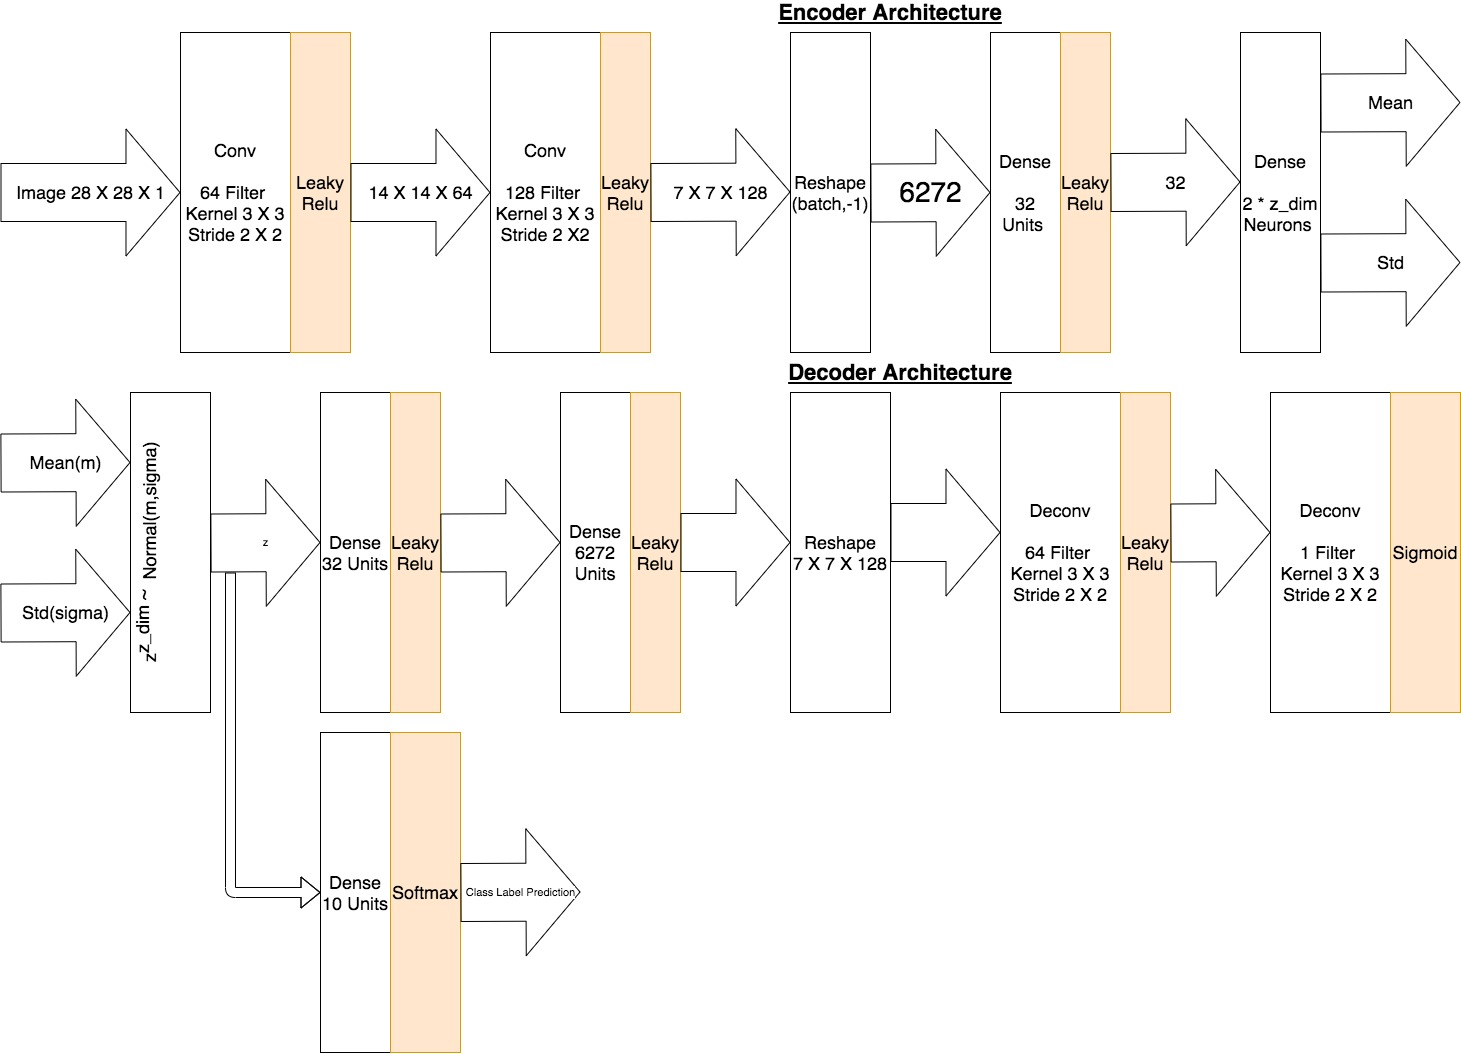
\includegraphics[width=3.5in]{vae_model_architecture_classification.jpg}
% where an .eps filename suffix will be assumed under latex, 
% and a .pdf suffix will be assumed for pdflatex; or what has been declared
% via  
\DeclareGraphicsExtensions.
\caption{Proposed model architecture}
\label{vae_architecture}
\end{figure}


\section{Results and Discussions} \label{results}
Figure \ref{reconstruction_accuracy} shows  the reconstruction accuracy of the variational autoencoder on the validation images after 5 epochs of training with $\gamma = 0$  and different values of latent vector dimension $z_{dim}$. It is observed that increasing $z_{dim}$ beyond 10 does not result in an increase in accuracy in the same proportion. This is because, the number of nodes in the 3rd layer were fixed at 32 which limits the representational capacity of that and all the subsequent layers.


\begin{figure}[!t]
\centering
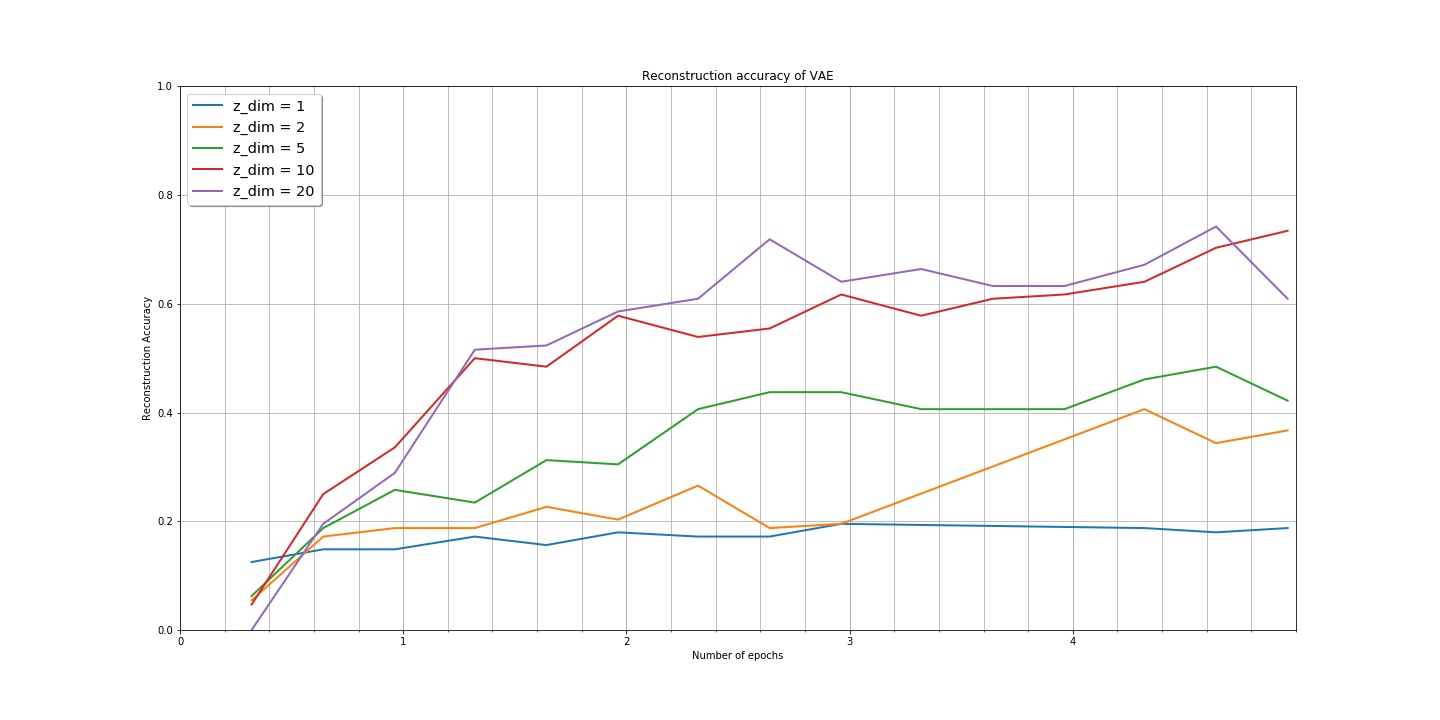
\includegraphics[width=4in]{reconstruction_accuracy.jpg}
\caption{Reconstruction accuracy of autoencoder on validation images with different values for the latent vector dimension  $z_{dim}$ and $\gamma = 0$}
\label{reconstruction_accuracy}
\end{figure}

Figure \ref{reconstruction_accuracy_sup_vs_unsup} shows that the reconstruction accuracy of VAE is improved significantly  (by 6 to 10 \%) when classification loss is added. The blue curve in figure shows the reconstruction accuracy when the latent vectors were clustered and a label were assigned to the reconstructed images corresponding to  cluster centers at the end of every epoch. Figure TODO add fig shows comparison of sample reconstructed images from validation set for normal autoencoder (unsupervised) versus the autoencoder with classification loss added.

\begin{figure}[!t]
\centering
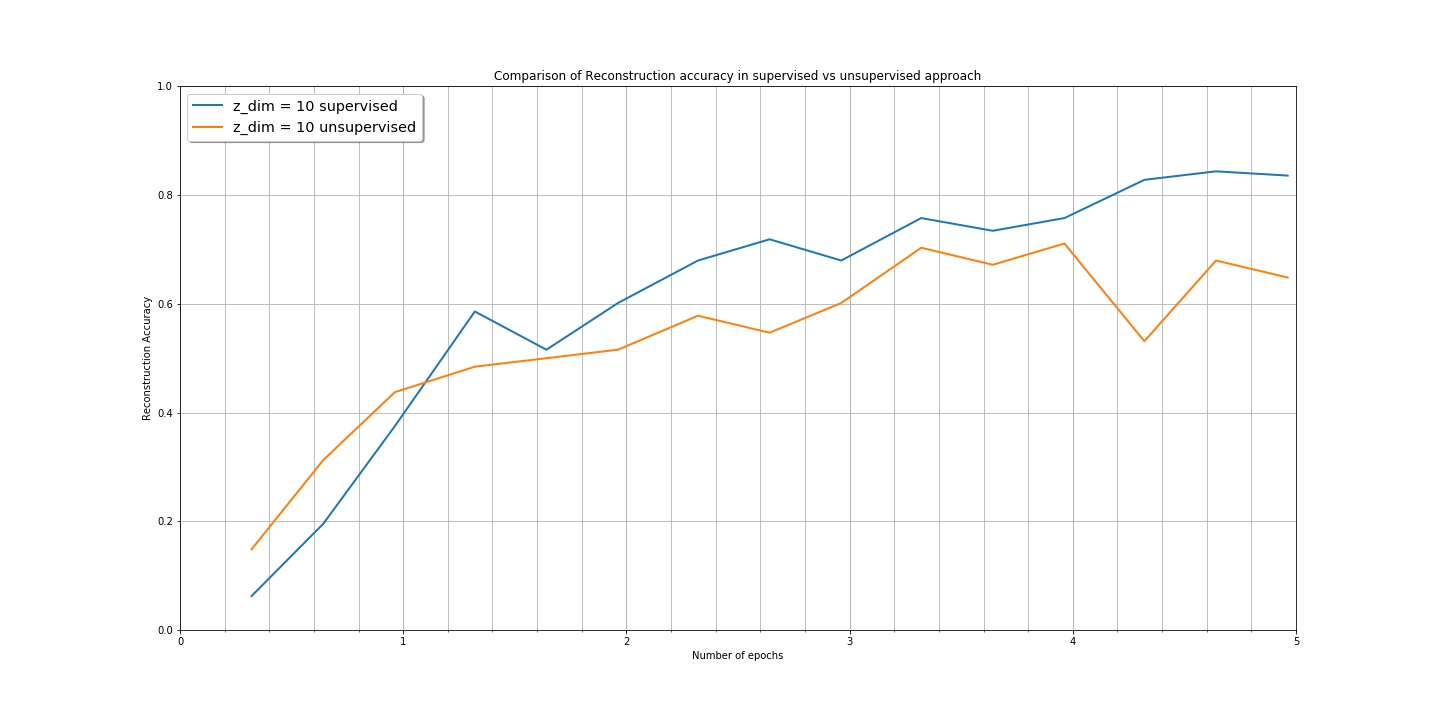
\includegraphics[width=4in]{reconstruction_accuracy_compare_supervised_vs_unsuprevised.jpg}
\caption{Comparison of reconstruction accuracy with and without classification loss }
\label{reconstruction_accuracy_sup_vs_unsup}
\end{figure}



%\colorbox{TODDO all link}

\subsubsection{Subsubsection Heading Here}
Subsubsection text here.


% An example of a floating figure using the graphicx package.
% Note that \label must occur AFTER (or within) \caption.
% For figures, \caption should occur after the \includegraphics.
% Note that IEEEtran v1.7 and later has special internal code that
% is designed to preserve the operation of \label within \caption
% even when the captionsoff option is in effect. However, because
% of issues like this, it may be the safest practice to put all your
% \label just after \caption rather than within \caption{}.
%
% Reminder: the "draftcls" or "draftclsnofoot", not "draft", class
% option should be used if it is desired that the figures are to be
% displayed while in draft mode.
%
%\begin{figure}[!t]
%\centering
%\includegraphics[width=2.5in]{myfigure}
% where an .eps filename suffix will be assumed under latex, 
% and a .pdf suffix will be assumed for pdflatex; or what has been declared
% via \DeclareGraphicsExtensions.
%\caption{Simulation Results.}
%\label{fig_sim}
%\end{figure}

% Note that IEEE typically puts floats only at the top, even when this
% results in a large percentage of a column being occupied by floats.


% An example of a double column floating figure using two subfigures.
% (The subfig.sty package must be loaded for this to work.)
% The subfigure \label commands are set within each subfloat command,
% and the \label for the overall figure must come after \caption.
% \hfil is used as a separator to get equal spacing.
% Watch out that the combined width of all the subfigures on a 
% line do not exceed the text width or a line break will occur.
%
%\begin{figure*}[!t]
%\centering
%\subfloat[Case I]{\includegraphics[width=2.5in]{box}%
%\label{fig_first_case}}
%\hfil
%\subfloat[Case II]{\includegraphics[width=2.5in]{box}%
%\label{fig_second_case}}
%\caption{Simulation results.}
%\label{fig_sim}
%\end{figure*}
%
% Note that often IEEE papers with subfigures do not employ subfigure
% captions (using the optional argument to \subfloat[]), but instead will
% reference/describe all of them (a), (b), etc., within the main caption.

% An example of a floating table. Note that, for IEEE style tables, the 
% \caption command should come BEFORE the table. Table text will default to
% \footnotesize as IEEE normally uses this smaller font for tables.
% The \label must come after \caption as always.
%
%\begin{table}[!t]
%% increase table row spacing, adjust to taste
%\renewcommand{\arraystretch}{1.3}
% if using array.sty, it might be a good idea to tweak the value of
% \extrarowheight as needed to properly center the text within the cells
%\caption{An Example of a Table}
%\label{table_example}
%\centering
%% Some packages, such as MDW tools, offer better commands for making tables
%% than the plain LaTeX2e tabular which is used here.
%\begin{tabular}{|c||c|}
%\hline
%One & Two\\
%\hline
%Three & Four\\
%\hline
%\end{tabular}
%\end{table}


% Note that IEEE does not put floats in the very first column - or typically
% anywhere on the first page for that matter. Also, in-text middle ("here")
% positioning is not used. Most IEEE journals use top floats exclusively.
% Note that, LaTeX2e, unlike IEEE journals, places footnotes above bottom
% floats. This can be corrected via the \fnbelowfloat command of the
% stfloats package.


\section{Conclusion} \label{conclusion}
The conclusion goes here.



% if have a single appendix:
%\appendix[Proof of the Zonklar Equations]
% or
%\appendix  % for no appendix heading
% do not use \section anymore after \appendix, only \section*
% is possibly needed

% use appendices with more than one appendix
% then use \section to start each appendix
% you must declare a \section before using any
% \subsection or using \label (\appendices by itself
% starts a section numbered zero.)
%


\appendices
\section{}

% you can choose not to have a title for an appendix
% if you want by leaving the argument blank
\section{}
Appendix two text goes here.

% use section* for acknowledgement
\section*{Acknowledgment}

The authors would like to thank...

% Can use something like this to put references on a page
% by themselves when using endfloat and the captionsoff option.
\ifCLASSOPTIONcaptionsoff
  \newpage
\fi

% trigger a \newpage just before the given reference
% number - used to balance the columns on the last page
% adjust value as needed - may need to be readjusted if
% the document is modified later
%\IEEEtriggeratref{8}
% The "triggered" command can be changed if desired:
%\IEEEtriggercmd{\enlargethispage{-5in}}

% references section

% can use a bibliography generated by BibTeX as a .bbl file
% BibTeX documentation can be easily obtained at:
% http://www.ctan.org/tex-archive/biblio/bibtex/contrib/doc/
% The IEEEtran BibTeX style support page is at:
% http://www.michaelshell.org/tex/ieeetran/bibtex/
%\bibliographystyle{IEEEtran}
% argument is your BibTeX string definitions and bibliography database(s)
%\bibliography{IEEEabrv,../bib/paper}
%
% <OR> manually copy in the resultant .bbl file
% set second argument of \begin to the number of references
% (used to reserve space for the reference number labels box)
\begin{thebibliography}{1}
\bibitem{resnet}
He, Kaiming, et al. "Deep residual learning for image recognition." Proceedings of the IEEE conference on computer vision and pattern recognition. 2016.

\bibitem{alexnet}
Krizhevsky, Alex, Ilya Sutskever, and Geoffrey E. Hinton. "Imagenet classification with deep convolutional neural networks." Advances in neural information processing systems 25 (2012): 1097-1105.
\bibitem{vggnet}
Simonyan, Karen, and Andrew Zisserman. "Very deep convolutional networks for large-scale image recognition." arXiv preprint arXiv:1409.1556 (2014)

\bibitem{vae}
Kingma, Diederik P., and Max Welling. "Auto-encoding variational bayes." arXiv preprint arXiv:1312.6114 (2013)

\bibitem{gan}
Goodfellow, Ian and Pouget-Abadie, Jean and Mirza, Mehdi and Xu, Bing and Warde-Farley, David and Ozair, Sherjil and Courville, Aaron and Bengio, Yoshua. "Generative adversarial nets". Advances in neural information processing systems.2014
\bibitem{laddernetwork}
Valpola, Harri. "From neural PCA to deep unsupervised learning." Advances in independent component analysis and learning machines. Academic Press, 2015. 143-171

\bibitem{mtl_2017_ruder}
Ruder, Sebastian. "An overview of multi-task learning in deep neural networks." arXiv preprint arXiv:1706.05098 (2017).

\bibitem{mtl_2020_michael}
Crawshaw, Michael. "Multi-Task Learning with Deep Neural Networks: A Survey." arXiv preprint arXiv:2009.09796 (2020).

\bibitem{mtl_zhang_2014}
Zhang, Zhanpeng, et al. "Facial landmark detection by deep multi-task learning." European conference on computer vision. Springer, Cham, 2014.

\bibitem{mtl_2016_dai}
Dai, Jifeng, Kaiming He, and Jian Sun. "Instance-aware semantic segmentation via multi-task network cascades." Proceedings of the IEEE Conference on Computer Vision and Pattern Recognition. 2016.

\bibitem{mtl_liu_2019}
Liu, Shikun, Edward Johns, and Andrew J. Davison. "End-to-end multi-task learning with attention." Proceedings of the IEEE Conference on Computer Vision and Pattern Recognition. 2019.

\bibitem{crnn}
Shi, Baoguang, Xiang Bai, and Cong Yao. "An end-to-end trainable neural network for image-based sequence recognition and its application to scene text recognition." IEEE transactions on pattern analysis and machine intelligence 39.11 (2017): 2298-2304.

\bibitem{faster_rcnn}
Ren, S., He, K., Girshick, R., and Sun, J. "Faster r-cnn: Towards real-time object detection with region proposal networks."  In Advances in neural information processing systems (2015) pp. 91-99.

\bibitem{yolo}
Redmon J, Divvala S, Girshick R, Farhadi A. "You only look once: Unified, real-time object detection. InProceedings of the IEEE conference on computer vision and pattern recognition"  (2016)  pp. 779-788.

\bibitem{dataset_marmot}
\url {http://www.icst.pku.edu.cn/cpdp/data/marmot_data.htm}

\bibitem{dataset_icdar}
\url{http://www.tamirhassan.com/html/competition.html}
\bibitem{mnist}
\url{http://yann.lecun.com/exdb/mnist/}

\bibitem{dataset_imagenet}
\url{http://www.image-net.org}

\end{thebibliography}

% biography section
% 
% If you have an EPS/PDF photo (graphicx package needed) extra braces are
% needed around the contents of the optional argument to biography to prevent
% the LaTeX parser from getting confused when it sees the complicated
% \includegraphics command within an optional argument. (You could create
% your own custom macro containing the \includegraphics command to make things
% simpler here.)
%\begin{IEEEbiography}[{\includegraphics[width=1in,height=1.25in,clip,keepaspectratio]{mshell}}]{Michael Shell}
% or if you just want to reserve a space for a photo:


% if you will not have a photo at all:
% insert where needed to balance the two columns on the last page with
% biographies
%\newpage

% You can push biographies down or up by placing
% a \vfill before or after them. The appropriate
% use of \vfill depends on what kind of text is
% on the last page and whether or not the columns
% are being equalized.

%\vfill

% Can be used to pull up biographies so that the bottom of the last one
% is flush with the other column.
%\enlargethispage{-5in}


% that's all folks
\end{document}


